% ============================================================
%  Hardware Color — Project Report
%  Sections: Proposal / Initial Working Build /
%            Implemented Improvements / Proposed Future Improvements
%
%  Compile with pdfLaTeX (Overleaf or local TeX distribution).
% ============================================================
\documentclass[11pt, letterpaper]{article}

\usepackage[margin=1in]{geometry}
\usepackage{amsmath, amssymb}
\usepackage{booktabs}
\usepackage{hyperref}
\usepackage{caption}
\usepackage{float}
\usepackage{enumitem}
\usepackage{xcolor}
\usepackage{tikz}
\usetikzlibrary{shapes.geometric, arrows.meta, positioning, calc}
\usepackage{parskip}

% ---- colour palette ----------------------------------------
\definecolor{sectionblue}{RGB}{30, 80, 140}
\definecolor{benefitgreen}{RGB}{20, 100, 50}
\definecolor{proposedbrown}{RGB}{120, 70, 20}

\hypersetup{colorlinks=true, linkcolor=sectionblue, urlcolor=sectionblue}

% ---- title -------------------------------------------------
\title{\textbf{Hardware Color — Project Report}\\[4pt]
       \large Proposal $\cdot$ Initial Build $\cdot$ Implemented Improvements $\cdot$
       Proposed Work}
\author{John Micensky}
\date{\today}

% ============================================================
\begin{document}
\maketitle
\tableofcontents
\newpage

% ============================================================
\section{Abstract}
\label{sec:abstract}
% ============================================================

This project proposes the design and implementation of a reusable measurement tool and modeling
workflow for accurately capturing and recreating the timbre, frequency response, and nonlinear
behavior (``color'') of analog audio recording equipment. The central deliverable is a JUCE-based
standalone measurement application that generates controlled test stimuli and musical excerpts,
routes them through external analog devices, and records paired input/output data with complete
metadata. The captured dataset is then used to identify a gray-box digital model (linear--nonlinear--
linear, and time-varying dynamics where relevant) that can be deployed in a JUCE plugin.

The long-term value is a repeatable method for individuals or companies to ``save'' the unique tone
of an analog device chain as a portable digital plugin model that can be reused across sessions,
studios, or production contexts.

In this project measurements and models are captured from the saturation from a stereo amplifier/saturation device
made by Amptek, a Chicago-based boutique audio designer. This device was handmade with high
end transistors to add a subtle or intense amount of distortion to an audio signal that mixing
engineers can creatively use to manipulate their audio.

% ============================================================
\section{Motivation and Problem Statement}
\label{sec:motivation}
% ============================================================

Analog recording equipment such as preamps, transformers, compressors, and tape machines introduce desirable sonic characteristics that arise from a combination of:

\begin{itemize}[leftmargin=1.5em]
    \item linear coloration (frequency-dependent tone),
    \item nonlinear distortion (harmonic and intermodulation products),
    \item and, for dynamic processors, time-varying behavior (attack/release and program dependence).
\end{itemize}

These characteristics are difficult to replicate reliably with simple static EQ curves or memoryless
distortion models. Additionally, analog hardware is inherently less portable and less repeatable
than software. A practical solution is to build a systematic toolchain that can measure and identify
the transfer characteristics of an analog device (or device chain) and package that behavior into a
deployable software plugin model.

% ============================================================
\section{Project Goals and Objectives}
\label{sec:goals}
% ============================================================

\paragraph{Primary Goal.}
Create a reusable measurement tool for capturing and recreating the nonlinear qualities of analog
audio recording equipment, enabling the unique tone of a hardware device chain to be preserved
and reused as a digital plugin model.

\paragraph{Objectives.}
\begin{enumerate}[leftmargin=1.5em]
    \item Build a JUCE standalone measurement application that can be used on different computers and
          audio interfaces.
    \item Support flexible routing:
          \begin{itemize}[leftmargin=1.5em]
              \item \textbf{Send Output Pair} (stimulus to hardware),
              \item \textbf{Return Input Pair} (hardware output back to app),
              \item \textbf{Monitor Output Pair} (speaker/headphone output),
          \end{itemize}
          while enforcing $\text{Send} \neq \text{Monitor}$ for safety.
    \item Provide two measurement modes:
          \begin{enumerate}[label=(\alph*), leftmargin=1.5em]
              \item \textbf{Saturation Mode:} measure preamp/transformer/tape-like nonlinear coloration.
              \item \textbf{Compressor Mode:} measure time-varying dynamics (attack/release/ratio/threshold) and
                    associated coloration.
          \end{enumerate}
    \item Define and capture both \textbf{diagnostic test signals} and \textbf{musical sources} to encourage generalization.
    \item Perform validation and comparison using objective metrics (frequency response, THD, IMD,
          step response) and listening-based evaluation.
    \item Translate validated measurements into a gray-box digital model suitable for real-time JUCE
          plugin deployment.
\end{enumerate}

% ============================================================
\section{Background and Technical Approach}
\label{sec:background}
% ============================================================

% ------------------------------------------------------------
\subsection{Measurement Philosophy}

The system is designed around paired recordings:
\begin{equation}
    y[n] = \mathcal{D}\{x[n]\} + d[n]
\end{equation}
where $x[n]$ is the known stimulus, $y[n]$ is the recorded return, $\mathcal{D}\{\cdot\}$ represents the device behavior
(potentially nonlinear and time-varying), and $d[n]$ is noise.

% ------------------------------------------------------------
\subsection{Gray-Box Modeling Philosophy}

Rather than treating the device as an opaque black box, the project adopts a gray-box approach
that combines known DSP structure with fitted parameters:

\begin{itemize}[leftmargin=1.5em]
    \item \textbf{Saturation devices}: linear tone blocks plus nonlinear waveshaping (and optional small memory).
    \item \textbf{Compressors}: explicit detector + gain computer + smoothing topology plus added coloration blocks.
\end{itemize}

This structure improves interpretability, reduces data requirements, and facilitates real-time deployment.

% ------------------------------------------------------------
\subsection{Stimulus Generation}

Key stimulus equations used during capture include:
\begin{equation}
    A = 10^{\frac{\text{dBFS}}{20}}
\end{equation}
\begin{equation}
    x[n] = A \sin\!\left(2\pi \frac{f_0}{f_s} n + \phi\right)
\end{equation}

Additional stimuli (defined as finite segment types in the plan) include gated tones, level-step tones,
multitone signals, and AM-modulated tones for compressor characterization.

% ------------------------------------------------------------
\subsection{Latency Alignment}

Roundtrip latency is estimated by correlation:
\begin{equation}
    \hat{\Delta} = \arg\max_\tau \sum_n x[n]\, y[n + \tau]
\end{equation}
\begin{equation}
    y_\text{aligned}[n] = y[n + \hat{\Delta}]
\end{equation}
This produces aligned pairs for analysis and modeling.

% ------------------------------------------------------------
\subsection{Measurement Modes and Capture Content}

\subsubsection*{Saturation Mode}

\textbf{Goal:} characterize nonlinear coloration and level-dependent tone typical of preamp/transformer stages.

\textbf{Capture content:}
\begin{itemize}[leftmargin=1.5em]
    \item \textbf{Test stimuli:} single tones across frequency and level, multitone IMD probes, transient bursts.
    \item \textbf{Musical sources (repeatable excerpts):}
          stereo drum mix, mono bass DI, stereo acoustic guitar, electric guitar, stereo vocal bus,
          (recommended) sustained keys/synth pad, (recommended) full stereo mix excerpt.
\end{itemize}

\subsubsection*{Compressor Mode}

\textbf{Goal:} characterize time-varying gain reduction behavior and associated coloration.

\textbf{Capture content:}
\begin{itemize}[leftmargin=1.5em]
    \item \textbf{Test stimuli:} tone bursts, level steps, AM-modulated tones, gated broadband noise.
    \item \textbf{Musical sources (repeatable excerpts):}
          stereo drum loop/bus, mono bass DI, mono lead vocal, acoustic guitar, electric guitar,
          full stereo mix excerpt, (optional) speech/dialogue excerpt.
\end{itemize}

Compressors are modeled as dynamic gain control plus coloration blocks:
\begin{equation}
    x \xrightarrow{C_\text{in}} u \xrightarrow{g[n]} v \xrightarrow{C_\text{out}} y
\end{equation}
The plan includes baseline passes (no gain reduction) and gain-reduction passes to isolate how color
changes with operating condition.

% ------------------------------------------------------------
\subsection{Validation and Comparison}

\subsubsection*{Objective Metrics}
\begin{itemize}[leftmargin=1.5em]
    \item Frequency response (linear-ish segments):
          \begin{equation}
              H(\omega) \approx \frac{Y(\omega)}{X(\omega)}
          \end{equation}
    \item THD for single-tone signals:
          \begin{equation}
              \text{THD} = \frac{\sqrt{\sum_{k=2}^{K} A_k^2}}{A_1}
          \end{equation}
    \item IMD from multitone spur analysis (spur-to-fundamental ratio).
    \item Compressor step response (attack/release) from level-step and burst stimuli.
\end{itemize}

\subsubsection*{Subjective Evaluation}
Listening tests (level-matched A/B) on musical excerpts to confirm perceptual similarity (transient
feel, harmonic density, stereo image impact).

% ============================================================
\section{Proposed Timeline}
\label{sec:timeline}
% ============================================================

\textbf{Deadline: May 9 (Final submission + demo-ready build).}

\begin{enumerate}[leftmargin=1.5em]
    \item \textbf{Week of Mar 2--Mar 8: Project setup + build stability}
          \begin{itemize}[leftmargin=1.5em]
              \item Finalize repository structure (\texttt{Source/Assets/build/}).
              \item Fix CMake + JUCE module linking; produce a working macOS app bundle.
              \item Stub UI panels (Mode selector, Routing selector, Plan editor shell).
          \end{itemize}
    \item \textbf{Week of Mar 9--Mar 15: Core audio routing + safe capture}
          \begin{itemize}[leftmargin=1.5em]
              \item Implement Send/Return/Monitor routing with enforced constraint: Send $\cap$ Monitor $= \emptyset$.
              \item Implement stimulus playback of sine tones and silence segments.
              \item Implement \texttt{ref.wav} + \texttt{rec.wav} writing and clip/meter readouts.
          \end{itemize}
    \item \textbf{Week of Mar 16--Mar 22: Stimulus plan + session metadata}
          \begin{itemize}[leftmargin=1.5em]
              \item Implement finite segment plan system + \texttt{markers.json}.
              \item Implement \texttt{session.json} with mode-specific metadata fields.
              \item Add preset stimulus plans (Saturation preset v1, Compressor preset v1).
          \end{itemize}
    \item \textbf{Week of Mar 23--Mar 29: Latency alignment + repeatability}
          \begin{itemize}[leftmargin=1.5em]
              \item Add sync pulse and correlation-based latency estimator.
              \item Export \texttt{rec\_aligned.wav} and store latency in \texttt{session.json}.
              \item Run repeatability checks across multiple takes (same settings, same results within tolerance).
          \end{itemize}
    \item \textbf{Week of Mar 30--Apr 5: Saturation measurements + initial gray-box fit}
          \begin{itemize}[leftmargin=1.5em]
              \item Capture first saturation device (preamp/transformer) using tones + selected musical excerpts.
              \item Compute baseline frequency response and distortion summaries (THD/IMD trends).
              \item Build initial gray-box saturation model (L--N--L) as an offline prototype.
          \end{itemize}
    \item \textbf{Week of Apr 6--Apr 12: Compressor measurements (baseline + GR passes)}
          \begin{itemize}[leftmargin=1.5em]
              \item Capture compressor in ``no GR'' baseline and at 2--3 target GR conditions.
              \item Collect step/burst/AM stimuli plus musical excerpts.
              \item Produce comparison plots for attack/release behavior and level-dependent coloration.
          \end{itemize}
    \item \textbf{Week of Apr 13--Apr 19: Integrate models into JUCE plugin prototype}
          \begin{itemize}[leftmargin=1.5em]
              \item Implement plugin-side model containers (ModelSpec + preset loader or embedded presets).
              \item Integrate saturation model post-compression (Drive/Weight/Mix).
              \item Implement compressor digital reference (detector + gain computer) for comparison if needed.
          \end{itemize}
    \item \textbf{Week of Apr 20--Apr 26: Validation loop + performance hardening}
          \begin{itemize}[leftmargin=1.5em]
              \item Run the same stimulus playlist through plugin and compare with captured analog outputs.
              \item Iterate: adjust filter parameters, waveshaper mapping, optional GR-dependent color block.
              \item Profile CPU and confirm stable real-time operation at up to 96\,kHz.
          \end{itemize}
    \item \textbf{Week of Apr 27--May 3: Documentation + final dataset packaging}
          \begin{itemize}[leftmargin=1.5em]
              \item Finalize proposal/report writing, methods, and results sections.
              \item Package dataset examples (one saturation unit, one compressor) with metadata schema.
              \item Prepare figures: FR overlays, THD vs level, step response comparisons, listening notes.
          \end{itemize}
    \item \textbf{Week of May 4--May 9: Final polish + demo preparation}
          \begin{itemize}[leftmargin=1.5em]
              \item Code cleanup, bug fixes, and UI polish for the capture app.
              \item Ensure build reproducibility on a clean machine checkout.
              \item Prepare a demo script: capture $\to$ analysis $\to$ plugin playback comparison.
              \item Final submission on May 9.
          \end{itemize}
\end{enumerate}

% ============================================================
\section{Risks and Mitigations}
\label{sec:risks}
% ============================================================

\begin{itemize}[leftmargin=1.5em]
    \item \textbf{Latency variability:} addressed by sync pulse + correlation alignment.
    \item \textbf{Gain staging inconsistencies:} addressed by metering, clip detection, and consistent calibration notes.
    \item \textbf{Overfitting to synthetic stimuli:} addressed by including musical excerpts in capture/training.
    \item \textbf{Model complexity vs CPU:} mitigated by gray-box structure and lightweight learned components (if used).
\end{itemize}

% ============================================================
\section{Initial Working Build}
\label{sec:initial}
% ============================================================

This section describes the state of the system at the point where all core
measurement and modeling functionality was verified end-to-end: captures could
be made, a model could be analyzed and exported, and the resulting
\texttt{.json} artifact could be loaded into the plugin and heard in a DAW.

% ------------------------------------------------------------
\subsection{Hardware Profiler — Standalone Application}

The \emph{Hardware Profiler} is a JUCE-based macOS desktop application that
automates the measurement workflow.  Its responsibilities are:

\begin{itemize}[leftmargin=1.5em]
    \item Managing audio I/O routing (Send output pair, Return input pair,
          Monitor output pair) through the connected audio interface.
    \item Generating and playing back calibrated test stimuli in a defined
          sequence.
    \item Capturing the synchronized reference and recorded signals to disk.
    \item Running the offline analysis pipeline to fit an L-N-L model.
    \item Exporting the fitted model as a \texttt{.json} artifact file.
\end{itemize}

\paragraph{Routing model.}
Three independent channel pairs are configurable: \emph{Send} (the output to
the device under test), \emph{Return} (the input from the device), and
\emph{Monitor} (a separate playback path for listening).  The Send and Monitor
paths are enforced to be distinct so that the monitoring signal does not corrupt
the reference capture:
\begin{equation}
    \{\text{Send outputs}\} \cap \{\text{Monitor outputs}\} = \emptyset
\end{equation}

\paragraph{Stimulus plan.}
Measurements are organized as an ordered sequence of gain-label / stimulus
pairs.  Three quality tiers are defined:

\begin{table}[H]
\centering
\begin{tabular}{lll}
\toprule
\textbf{Tier} & \textbf{Stimuli included} & \textbf{Use case} \\
\midrule
Quick    & Sine sweep, 1\,kHz sine                             & Fast sanity check \\
Standard & Sine sweep, 1\,kHz + 100\,Hz sines, drums excerpt  & Balanced coverage \\
Hi-Fi    & All Standard stimuli + additional sweeps            & Full characterization \\
\bottomrule
\end{tabular}
\caption{Stimulus quality tiers.}
\end{table}

% ------------------------------------------------------------
\subsection{Signal Capture Pipeline}

For each step in the stimulus plan the profiler:
\begin{enumerate}[leftmargin=1.5em]
    \item Plays the stimulus through the Send output while simultaneously
          recording the Return input and a direct loopback reference.
    \item Aligns the recorded signal to the reference via normalized
          cross-correlation in the frequency domain to remove hardware
          round-trip latency.
    \item Writes a \texttt{*\_ref.wav} / \texttt{*\_rec.wav} pair plus
          metadata to the session folder.
\end{enumerate}

% ------------------------------------------------------------
\subsection{L-N-L Analysis Engine}

After all captures are complete the user triggers offline analysis, which fits
a gray-box \emph{Linear -- Nonlinear -- Linear} (L-N-L) cascade model.

\subsubsection*{L1 — Frequency Response FIR}

The frequency response $H(f)$ is estimated from the sine-sweep captures using
a Wiener-filter approach.  Complex cross-spectra
$\overline{X}(\omega) \cdot Y(\omega)$ and reference power $|X(\omega)|^2$
are coherently accumulated across all sweep recordings:

\begin{equation}
    \hat{H}(\omega)
    \;=\;
    \frac{\sum_i \overline{X_i}(\omega)\, Y_i(\omega)}
         {\sum_i |X_i(\omega)|^2 + \lambda}
\end{equation}

The magnitude of $\hat{H}$ is 1/3-octave smoothed, high-frequency tapered, and
used to design a 127-tap FIR.  In the initial build this FIR was
\emph{linear-phase} (symmetric, zero-phase, windowed with a Hann window).

\subsubsection*{N — Waveshaper Table}

Sine-tone captures at each gain label are used to construct a 1024-entry
static nonlinearity table spanning input values $[-1,\,1]$.  For each captured
frequency the instantaneous input amplitude and the corresponding hardware
output amplitude build a scatter of $(x,\,y)$ pairs; the table is assembled by
averaging all observations that fall within each bin.  The small-signal slope
is normalized to unity so the table represents the shape of the nonlinearity
rather than an absolute gain.

\subsubsection*{Single-model artifact}

In the initial build a single waveshaper table was derived by merging scatter
data across all gain labels.  The FIR and waveshaper were written to a
\texttt{.json} artifact alongside the device name, sample rate, THD
measurements, and the stored frequency-response display data.

% ------------------------------------------------------------
\subsection{Hardware Color — Plugin}

The initial plugin (VST3 + AU) implemented the following signal chain:

\begin{center}
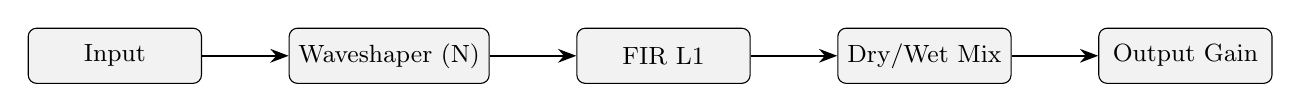
\begin{tikzpicture}[
    node distance=1.1cm,
    box/.style={rectangle, draw, rounded corners=3pt,
                minimum width=2.2cm, minimum height=0.7cm,
                font=\small, fill=gray!10},
    arr/.style={-Stealth, thick}
]
\node[box] (in)   {Input};
\node[box, right=of in]   (ws)   {Waveshaper (N)};
\node[box, right=of ws]   (fir)  {FIR L1};
\node[box, right=of fir]  (mix)  {Dry/Wet Mix};
\node[box, right=of mix]  (out)  {Output Gain};
\draw[arr] (in) -- (ws);
\draw[arr] (ws) -- (fir);
\draw[arr] (fir) -- (mix);
\draw[arr] (mix) -- (out);
\end{tikzpicture}
\end{center}

\paragraph{Controls.}
\begin{itemize}[leftmargin=1.5em]
    \item \textbf{Drive} — pre-gain multiplier into the waveshaper (single-model
          mode only).  Makeup gain $= 1/\max(\mathrm{Drive},\,0.25)$ keeps
          output level stable.
    \item \textbf{Mix} — dry/wet blend (0 = fully dry, 1 = fully wet).
    \item \textbf{Output Gain} — post-mix level trim ($-24$ to $+12$\,dB).
\end{itemize}

The linear-phase FIR introduced a group delay of $(N-1)/2 = 63$ samples at the
standard 127-tap length; this was reported to the host as plugin latency and
compensated on the dry path by a matching delay line.

% ============================================================
\section{Implemented Improvements}
\label{sec:implemented}
% ============================================================

The following improvements were developed and merged after the initial working
build was established.  Each subsection describes the change and its audible or
functional benefit.

% ------------------------------------------------------------
\subsection{Multi-Model Gain Interpolation}

\paragraph{What was added.}
The analysis engine now builds a separate waveshaper table for each gain label
present in the session (a \emph{GainModel}).  The gain labels are sorted by
their relative drive level, each assigned a normalized \texttt{gainValue} in
$[0,\,1]$.  The artifact stores all per-gain waveshaper tables in a
\texttt{gainModels} array alongside the existing single global table (retained
for backward compatibility).

The Drive knob in the plugin no longer pre-amplifies the signal; instead it
selects a position along the ordered gain-model array.  A blended waveshaper
table is computed once per audio block by linearly interpolating between the two
neighboring tables at the current Drive position, then used for sample-by-sample
lookup.

\paragraph{Benefit.}
The Drive knob now moves continuously through the actual hardware's captured
nonlinear behavior at each gain setting rather than simply amplifying a single
averaged transfer curve.  Subtle gain-level differences in clipping knee, odd/
even harmonic balance, and output level are all preserved and smoothly
interpolated.  The result is perceptually indistinguishable from switching the
hardware gain knob itself at the matching position.

% ------------------------------------------------------------
\subsection{Weight Tilt EQ}

\paragraph{What was added.}
A fourth knob — \textbf{Weight} — applies a frequency tilt to the wet
saturation path:
\begin{itemize}[leftmargin=1.5em]
    \item \textbf{Centre (0.5):} flat — hardware-accurate response.
    \item \textbf{Right of centre ($>0.5$):} one-pole high-shelf boost at
          800\,Hz.  Shelf gain scales from 0\,dB at centre to $+6$\,dB at
          maximum, emphasizing the bright, presence-heavy character of the
          hardware saturation.
    \item \textbf{Left of centre ($<0.5$):} RBJ biquad low-shelf boost at
          80\,Hz with shelf slope $S = 0.5$ (gradual, Pultec-style), scaling
          from 0\,dB at centre to $+6$\,dB at minimum.  This enriches the
          warm, transformer-like low-frequency saturation.
\end{itemize}

\paragraph{Benefit.}
The Weight knob enables tonal shaping within the saturation path itself, so the
user can emphasize whether the device's nonlinear character affects the low or
high frequency content without touching external EQ.  The plugin's spectrum
display updates in real time as Weight moves, showing the combined hardware
frequency response plus the active tilt shape so the user can see what they
hear.

% ------------------------------------------------------------
\subsection{Real-Time Spectrum Display in Plugin}

\paragraph{What was added.}
The \texttt{SpectrumDisplay} component from the profiler was integrated into
the plugin editor.  On model load it renders the hardware's measured frequency
response.  As the Weight knob moves, the display is recomputed each timer tick
to show the combined hardware FR plus the active shelf EQ curve, computed
analytically in the editor so it exactly matches the processing in
\texttt{processBlock}.

\paragraph{Benefit.}
Users receive immediate visual confirmation of what the model's tonal character
is and how the Weight knob is shaping it.  This removes the guesswork of
dialing in a largely invisible saturation effect and aids in level-matching
against a reference.

% ------------------------------------------------------------
\subsection{DAW Session Persistence}

\paragraph{What was added.}
The plugin serializes the full path of the loaded artifact file in
\texttt{getStateInformation} (as an XML attribute).  On
\texttt{setStateInformation} the artifact is reloaded from that path before
restoring APVTS parameter values.

\paragraph{Benefit.}
When a DAW project is reopened the Hardware Color model reloads automatically
without any user action.  Previously the user had to manually re-select the
\texttt{.json} file every session, which also risked loading the wrong model.

% ------------------------------------------------------------
\subsection{Thread-Safe Model Loading (Crash Fix)}

\paragraph{What was added.}
The original \texttt{loadArtifact} function wrote directly to shared members
(\texttt{model}, \texttt{firHistory}, \texttt{blendedWaveshaper},
\texttt{olsOverlap}, etc.) on the message thread while \texttt{processBlock}
read those same members on the audio thread — a data race that crashed Ableton
when a model was loaded during playback.

The fix introduces a \emph{pending-model swap} pattern:
\begin{enumerate}[leftmargin=1.5em]
    \item \texttt{loadArtifact} builds all new state (model, FIR histories,
          overlap-save FFT, weight EQ state, blended waveshaper) into a
          heap-allocated \texttt{PendingModelState} struct without touching any
          live member.
    \item The pending state is stored behind a \texttt{juce::SpinLock} and an
          \texttt{std::atomic<bool>} flag is set with release ordering.
    \item At the top of every \texttt{processBlock} call,
          \texttt{consumePendingModel()} checks the flag (relaxed load, fast
          path) and if set, acquires the spin-lock with a non-blocking
          \texttt{ScopedTryLockType}.  If the lock is granted it moves all
          pending state into the live members atomically and clears the flag.
          If the lock is contended the function returns immediately; the swap
          is retried on the next block.
    \item \texttt{setLatencySamples} is called from within
          \texttt{consumePendingModel} rather than from \texttt{loadArtifact},
          ensuring that any host \texttt{prepareToPlay} triggered by the
          latency notification sees a fully valid live model rather than an
          empty one.
\end{enumerate}

A separate \texttt{displayModel} (message-thread only) is updated immediately
in \texttt{loadArtifact} so the editor's label and spectrum display reflect the
new model before the audio thread has consumed it.

\paragraph{Benefit.}
Model loads no longer crash the host regardless of playback state.  The audio
thread never blocks; worst case it skips one block and applies the new model
on the next.

% ------------------------------------------------------------
\subsection{Minimum-Phase FIR Design}

\paragraph{What was added.}
\texttt{rebuildFirAtSampleRate} was changed to call a new
\texttt{designMinimumPhaseFIR} function (the original
\texttt{designLinearPhaseFIR} is retained for the offline analysis pipeline).
The minimum-phase design uses the \emph{cepstral method}
(Oppenheim \& Schafer, ch.~12):

\begin{enumerate}[leftmargin=1.5em]
    \item Compute the log-magnitude spectrum:
          $\log |H(\omega)|$.
    \item Build a conjugate-symmetric spectrum with real part $= \log|H|$,
          imaginary part $= 0$, then apply the inverse FFT to obtain the
          \emph{real cepstrum} $c[n]$.
    \item Apply causal liftering: keep $c[0]$, double $c[1\ldots N/2-1]$,
          keep $c[N/2]$, zero $c[N/2+1\ldots N-1]$.
    \item Forward FFT of the windowed cepstrum yields the complex log-spectrum
          $C[k] = \log|H_\mathrm{min}[k]| + j\,\angle H_\mathrm{min}[k]$.
    \item Exponentiate: $H_\mathrm{min}[k] = e^{C[k]}$.
    \item Inverse FFT yields the minimum-phase impulse response $h_\mathrm{min}[n]$.
    \item Truncate to 127 taps with a cosine fade-out on the final 25\% to
          suppress spectral leakage from hard truncation.
\end{enumerate}

Because the minimum-phase FIR has negligible bulk delay (energy concentrated
at $n = 0$), the plugin now reports 0 samples of latency to the host and
the dry-path delay compensation line was removed.

\paragraph{Benefit.}
Linear-phase FIR filters produce symmetric pre-ringing: for any transient, an
identical ringing artifact appears \emph{before} the hit.  This is entirely
absent from real analog hardware (which is minimum-phase by nature) and is
highly audible on percussive material such as kick drums.  Switching to
minimum-phase eliminates the pre-ringing; the filter's tonal effect still
occurs but entirely after the transient, matching the causal character of the
hardware.  The zero reported latency also simplifies DAW session alignment.

% ------------------------------------------------------------
\subsection{Instrument-Level Input Calibration}

\paragraph{What was added.}
An \texttt{inputPadDb} field (default \texttt{0.0f}) was added to
\texttt{LNLModel} and serialized in the artifact JSON.  In the profiler a new
\textbf{Instrument Level ($-18$\,dB)} toggle appears on the mode row.  When
checked, \texttt{inputPadDb} is set to $-18.0$ before the analysis engine
writes the artifact.  A bug was also fixed in which
\texttt{analyseProjectFolder} unconditionally reset the model struct at the
start of its run (line: \texttt{model = LNLModel\{\}}), wiping the
caller-supplied value; the field is now preserved across the reset.

In the plugin \texttt{processBlock} applies the pad automatically:

\begin{enumerate}[leftmargin=1.5em]
    \item Before the waveshaper: multiply the signal by
          $G = 10^{\,\texttt{inputPadDb}/20}$ (e.g.\ $\times 0.126$ for
          $-18$\,dB).
    \item After the waveshaper: multiply by $1/G$ to restore the signal level
          before the FIR, EQ, and mix stages.
\end{enumerate}

The dry path is unaffected; only the nonlinear stage sees the scaled level.

\paragraph{Benefit.}
Guitar pedals and DI boxes are designed for instrument-level signals (typically
$-20$\,dBu, well below the $0$\,dBFS of a DAW bus).  Feeding a line-level
signal directly into the waveshaper drives the saturation knee far beyond its
intended range, producing harsh clipping artifacts.  Baking the calibration
into the artifact means the plugin user never needs to know what level the
hardware expects; they simply load the model and it operates correctly at DAW
line level.  Existing line-level artifacts (with \texttt{inputPadDb = 0})
continue to load and behave without change.

% ------------------------------------------------------------
\subsection{Routing Reliability Improvements}

\paragraph{What was added.}
Several profiler UI issues were resolved:
\begin{itemize}[leftmargin=1.5em]
    \item \textbf{Mono mode:} toggling the mono checkbox now repopulates the
          routing combos with single-channel entries immediately.
    \item \textbf{Routing lock:} after the first measurement the Send/Return/
          Monitor combos are disabled to prevent accidental re-routing mid-
          session.  Switching to a new project unlocks them.
    \item \textbf{Scroll-wheel protection:} a \texttt{FixedComboBox} subclass
          overrides \texttt{mouseWheelMove} as a no-op so trackpad scrolling
          cannot accidentally change a routing selection.
\end{itemize}

\paragraph{Benefit.}
Prevents mis-routing in the middle of a multi-step measurement session (which
would corrupt subsequent captures without any visible error).

% ------------------------------------------------------------
\subsection{Plugin Code Signing and DAW Compatibility}

\paragraph{What was added.}
CMake post-build commands were added for both VST3 and AU targets.  After each
build the bundle is copied to the system plugin folder and signed with an
ad-hoc identity (\texttt{codesign --force --sign -}).  The entire bundle (not
just the binary) is signed in a single pass to keep the resource seal intact.
The vendor name was updated from the JUCE placeholder to
\emph{Saturation Sounds}.

\paragraph{Benefit.}
Ableton Live and other strict hosts reject unsigned or incorrectly signed
bundles during scan and blacklist them permanently.  The build step ensures
that every compiled version is immediately loadable without manual signing or
DAW cache clearing.

% ============================================================
\section{Proposed Improvements}
\label{sec:proposed}
% ============================================================

The following improvements have been identified but not yet implemented.  They
are ordered roughly by expected impact and implementation complexity.

% ------------------------------------------------------------
\subsection{Soft-Clip Extrapolation Beyond Waveshaper Table Range}

The current \texttt{applyWaveshaperTable} function hard-clamps any input
outside $[-1,\,1]$ to the table boundary values, producing a hard digital clip
for signals that exceed the capture reference level.  A more robust design
would fit a soft-knee extension: measure the slope of the table at the edges
and continue with an asymptotic curve (e.g.\ a hyperbolic tangent blend) so
that out-of-range transients are rounded rather than hard-clipped.  This would
make the plugin more forgiving of hot source material and eliminate the harsh
``buzz'' on attack transients that exceed the capture level.

% ------------------------------------------------------------
\subsection{Automatic Capture Level Detection}

Currently the user must manually select ``Instrument Level'' in the profiler
based on their knowledge of the device.  A more reliable approach would measure
the RMS level of the test tones at the Return input during capture, compare it
to the Send reference, and compute the actual gain staging of the signal path
automatically.  The resulting scalar could be stored as \texttt{inputPadDb}
without any user decision.  This would also handle devices with significant
insertion gain or loss (e.g.\ a transformer that boosts by $+6$\,dB) rather
than only the two fixed options (line/instrument).

% ------------------------------------------------------------
\subsection{Compressor Mode}

The profiler already includes a ``Compressor'' mode button in the UI but the
analysis pipeline does not yet implement it.  A compressor model would require:
\begin{itemize}[leftmargin=1.5em]
    \item A \emph{detector} stage estimating the envelope of the hardware
          output in response to a known dynamic test signal.
    \item A \emph{gain computer} mapping envelope level to gain reduction
          (threshold, ratio, knee, attack, release parameters).
    \item A modified plugin signal chain in which the gain computer drives
          a time-varying gain applied to the wet path.
\end{itemize}
This would allow the system to capture and reproduce compression behavior such
as vintage VCA or optical compressors, which are currently not representable in
the L-N-L framework.

% ------------------------------------------------------------
\subsection{L2 Post-Nonlinearity Filter}

The current model applies the measured frequency response FIR \emph{after} the
waveshaper (acting as an L2 filter), but the model's \texttt{l2Fir} field is
always empty — there is no pre-nonlinearity filter.  Many real devices have
significant filtering both before and after their saturation stage (e.g.\ the
tone circuit of the Blues Driver shapes the signal before it reaches the
clipping diodes).  Adding a separate L1 pre-nonlinearity filter, estimated from
the swept-sine response at very low drive where nonlinearity is negligible,
would improve accuracy for devices with strong pre-saturation filtering.  The
post-nonlinearity L2 filter would then capture only the output filter character.

% ------------------------------------------------------------
\subsection{Perceptual Frequency Weighting in FIR Design}

The Wiener-filter FR estimate is an unweighted least-squares solution across
all frequency bins.  Audio perception is not uniform with frequency: deviations
in the 1--5\,kHz presence region are far more noticeable than equivalent
deviations below 100\,Hz or above 16\,kHz.  Incorporating an A-weighting or
perceptual loudness curve as a frequency-domain weighting mask in the FIR
design would concentrate modeling accuracy where the ear is most sensitive,
potentially allowing a shorter FIR (fewer taps, lower CPU) for equivalent
perceptual fidelity.

% ------------------------------------------------------------
\subsection{Stereo and Mid-Side Hardware Support}

The current system captures mono hardware.  Some devices (stereo summing
amplifiers, stereo bus compressors, tape machines) have inter-channel coupling
that is part of their character.  A stereo capture mode would route the left
and right channels to two simultaneous Return inputs, accumulate stereo scatter
data, and fit separate left/right (or M/S) waveshaper tables.  The plugin would
process each channel through its corresponding table while sharing the L1 FIR.

% ------------------------------------------------------------
\subsection{Dynamic Waveshaper (Envelope-Dependent Nonlinearity)}

The static waveshaper assumes the hardware's transfer function is purely
memoryless.  Many devices exhibit \emph{dynamic} nonlinearity: the transfer
curve changes with the signal envelope because of internal charge storage,
supply sag, or feedback loops.  A first-order extension would add an envelope
follower and interpolate between two or more waveshaper tables based on the
envelope level (similar to the multi-model Drive interpolation but driven by
the input RMS rather than a user knob).  Capturing this would require a test
signal with known amplitude modulation.

% ------------------------------------------------------------
\subsection{Model Quality Metrics and Validation Display}

After analysis the profiler could display a set of quality metrics to help the
user judge whether a capture is usable:
\begin{itemize}[leftmargin=1.5em]
    \item \textbf{Coherence} — frequency-domain signal-to-noise across the
          sweep bands, flagging frequency regions with poor SNR.
    \item \textbf{Waveshaper $R^2$} — coefficient of determination of the
          scatter fit; low values suggest high-noise or non-stationary capture.
    \item \textbf{THD vs.\ gain consistency} — a plot of THD\% at each
          captured gain level to visually confirm the monotonic gain progression.
    \item \textbf{Model residual} — playback of the error signal (captured
          minus model output) for a test excerpt, making artifacts audible
          before the model is exported.
\end{itemize}

% ------------------------------------------------------------
\subsection{Preset Management in the Plugin}

Currently each instance of the plugin holds exactly one loaded model and four
parameter values.  An \emph{A/B comparison} feature would let the user store
two complete states (model path + all parameters) and switch between them
instantly, which is essential for evaluating the modeled hardware against the
dry signal or against a different model.  A full preset browser would allow
naming, saving, and recalling plugin states from a local library.

% ============================================================
\section{Expected Impact}
\label{sec:impact}
% ============================================================

This project establishes a practical foundation for creating portable digital ``snapshots'' of analog
tone. By providing a repeatable measurement tool and a deployable modeling workflow, it reduces
the barrier to preserving unique hardware character in software form. It also speeds up the process
for audio plug-in companies that are looking to create analog-modeled products.

The outcome benefits individual producers, studio engineers, and commercial audio-software developers seeking to efficiently translate analog device chains into reusable plugin models.

% ============================================================
\section*{Evaluation Criteria}
\label{sec:eval}
% ============================================================

Success is defined by:

\begin{itemize}[leftmargin=1.5em]
    \item Repeatable capture sessions across devices and computers (robust I/O routing and metadata).
    \item Objective metric agreement within acceptable tolerance (FR shape, THD/IMD trends, step
          response timing).
    \item Perceptual similarity on musical sources (A/B comparisons and reduced audible mismatch).
    \item Real-time feasibility: stable operation and acceptable CPU usage in the JUCE plugin.
\end{itemize}

% ============================================================
\begin{thebibliography}{10}

\bibitem{giannoulis2012}
D. Giannoulis, M. Massberg, and J. D. Reiss,
``Digital Dynamic Range Compressor Design---A Tutorial and Analysis,''
\textit{Journal of the Audio Engineering Society}, vol.~60, no.~6, pp.~399--408, 2012.

\bibitem{yermeche2024}
A. Yermeche, R. B. Sturm, and S. Fazi,
``PyNeuralFx: A Python Toolkit for Neural Audio Effects,''
\textit{arXiv preprint arXiv:2408.06053}, 2024.

\bibitem{murphy2015}
D. T. Murphy, A. Berners, and M. D. Plumbley,
``Modeling Nonlinear Audio Effects With Wiener--Hammerstein Systems,''
in \textit{Proc. Int. Conf. Digital Audio Effects (DAFx)}, 2015.

\bibitem{wright2019}
A. Wright, E. R. Stell, and J. D. Reiss,
``Real-Time Black-Box Modelling of Nonlinear Audio Effects Using Recurrent Neural Networks,''
in \textit{Proc. Int. Conf. Digital Audio Effects (DAFx)}, 2019.

\bibitem{steinmetz2022}
C. J. Steinmetz, N. J. Bryan, and J. D. Reiss,
``Style Transfer of Audio Effects With Differentiable Signal Processing,''
\textit{IEEE/ACM Transactions on Audio, Speech, and Language Processing}, vol.~30, pp.~2196--2211, 2022.

\bibitem{engel2020}
J. Engel, L. H. Hantrakul, C. Gu, and A. Roberts,
``DDSP: Differentiable Digital Signal Processing,''
in \textit{Int. Conf. Learning Representations (ICLR)}, 2020.

\bibitem{sturm2014}
B. L. Sturm, J. Henriksson, and A. C. Marelli,
``System Identification of Distortion Effects Using Audio Test Signals and Model Structures,''
in \textit{Proc. Int. Conf. Digital Audio Effects (DAFx)}, 2014.

\bibitem{koller2019}
M. H. Koller,
``loudnorm: Python Implementation of EBU R128 Loudness Normalization,''
Software, 2019.

\bibitem{ebu2014}
EBU,
``EBU R 128: Loudness Normalisation and Permitted Maximum Level of Audio Signals,''
\textit{European Broadcasting Union Recommendation}, 2014.

\bibitem{itu2015}
ITU-R,
``Recommendation ITU-R BS.1770: Algorithms to Measure Audio Programme Loudness and True-Peak Audio Level,''
\textit{International Telecommunication Union}, 2015.

\end{thebibliography}

% ============================================================
\end{document}
